\documentclass[11pt]{article}
\usepackage[margin=0.5in,landscape]{geometry}
\usepackage{amsmath,amssymb,amsthm}
\usepackage{stmaryrd}
\usepackage{mathpartir}
\usepackage{xcolor}
\usepackage{adjustbox}
\usepackage{tikz}
\usetikzlibrary{arrows.meta,positioning,calc,fit,backgrounds}

\newtheorem*{lemma}{Lemma}

% lambda-PR (Koronkevich & Bowman, ICFP 2025)
\newcommand{\Nat}{\mathsf{Nat}}
\newcommand{\Unit}{\mathsf{Unit}}
\newcommand{\tRef}{\mathsf{Ref}\,}
\newcommand{\Type}[1]{\mathsf{Type}_{#1}}
\newcommand{\arr}[1]{\xrightarrow{#1}}
\newcommand{\new}{\mathsf{new}\,}
\newcommand{\deref}{!\,}
\newcommand{\assign}{\mathrel{:=}}
\newcommand{\unit}{\langle\rangle}
\newcommand{\lam}[2]{\lambda #1{:}#2.\,}
\newcommand{\maxlevel}{\operatorname{max-level}}
\newcommand{\FV}{\mathit{FV}}
\newcommand{\klet}{\mathsf{let}\ }
\newcommand{\kin}{\ \mathsf{in}\ }
% promises: type, introduction, forcing
\newcommand{\Prom}[2]{\lceil #2 \rceil^{#1}}
\newcommand{\prom}[1]{\lceil #1 \rceil}
\newcommand{\frc}[1]{\lfloor #1 \rfloor}
% source STLC
\newcommand{\snat}{\mathsf{nat}}
\newcommand{\slam}[1]{\lambda #1.\,}
% translation
\newcommand{\tr}[1]{\llbracket #1 \rrbracket}
\newcommand{\trc}[1]{\llbracket #1 \rrbracket^{\mathsf{c}}}
% rule labels; \bad highlights the failing side condition
\newcommand{\rn}[1]{\textsc{#1}}
\newcommand{\bad}[1]{\colorbox{red!15}{$#1$}}
\newcommand{\good}[1]{\colorbox{green!15}{$#1$}}
% logical relation over worlds
\newcommand{\Vrel}[2]{\mathcal{V}\llbracket #1 \rrbracket(#2)}
\newcommand{\Erel}[2]{\mathcal{E}\llbracket #1 \rrbracket(#2)}
\newcommand{\Grel}[2]{\mathcal{G}\llbracket #1 \rrbracket(#2)}
\newcommand{\last}[1]{\mathit{last}(#1)}
\newcommand{\ext}{\sqsupseteq}
\newcommand{\cfg}[2]{\langle #1 \mid #2 \rangle}
\newcommand{\evals}[5]{\cfg{#1}{#2} \Downarrow \cfg{#3}{#4} \mathrel{\triangleright} #5}
\newcommand{\fresh}{\mathit{fresh}}
\newcommand{\Val}{\mathit{Val}}
% Typeset a derivation on a wide canvas so mathpartir never wraps premises,
% then shrink it to the line width if needed.
\newcommand{\tree}[1]{%
  \begin{center}
  \adjustbox{max width=\linewidth}{\hsize=60cm \linewidth=60cm $#1$}
  \end{center}}

\title{A call-by-need STLC program with no stratified model}
\date{}

\begin{document}
\maketitle

\section{The counterexample}

In call-by-need STLC, consider
\[
  P \;\triangleq\; \slam{g} g\,(\slam{n} g\,(\slam{m} m))
  \;:\; ((\snat \to \snat) \to \snat) \to \snat
\]
$P$ calls $g$ twice, and the outer call passes a function that itself calls
$g$. Both calls go through $g$'s single, shared cell. We show that $P$ has no
stratified translation, so no program that uses it has one either.

\section{Translation to $\lambda_{\mathrm{PR}}$}

\paragraph{Promises.}
A promise $\prom{e}$ is a memoizing thunk: a reference holding a suspended
computation. Forcing it, $\frc{x}$, runs the computation and overwrites the
reference with its value. $\mathsf{let}$ and sequencing stand for the usual
$\beta$-redexes. Forcing is only ever applied to variables.

\medskip
\noindent\quad
$\begin{array}{@{}l@{\;\;\triangleq\;\;}l@{}}
  \Prom{k}{\tau} & \tRef (\Unit \arr{k} \tau) \\
  \prom{e} & \new (\lam{\_}{\Unit} e) \\
  \frc{x} & \klet v = (\deref x)\,\unit \kin x \assign (\lam{\_}{\Unit} v);\ v
\end{array}$
\medskip

\begin{lemma}[Promises]
  The following rules are admissible:
  \begin{mathpar}
    \inferrule*[right=\rn{Promise}]
      {\tau :: \Type{i} \\ k \geq i}
      {\Prom{k}{\tau} :: \Type{k+1}}
    \and
    \inferrule*[right=\rn{Promise}]
      {\Gamma \vdash e : \tau \\ k \geq \maxlevel(\FV(e), \tau)}
      {\Gamma \vdash \prom{e} : \Prom{k}{\tau}}
    \and
    \inferrule*[right=\rn{Force}]
      {x : \Prom{k}{\tau} \in \Gamma}
      {\Gamma \vdash \frc{x} : \tau}
  \end{mathpar}
\end{lemma}
\begin{proof}[Sketch]
  Kinding is \rn{Arr} (with $\Unit :: \Type{0}$) followed by \rn{Ref}. Typing a
  promise is \rn{Lam} followed by \rn{New}, where the $\lambda$'s side
  condition is
  \[
    k \;\geq\; \maxlevel(\FV(e), \Unit, \tau) \;=\; \maxlevel(\FV(e), \tau).
  \]
  For forcing, the write-back $\lam{\_}{\Unit} v : \Unit \arr{k} \tau$ needs
  $k \geq \maxlevel(\{v\}, \Unit, \tau) = \maxlevel(\tau)$, which kinding
  already guarantees. The levels on the $\beta$-redexes that encode
  $\mathsf{let}$ and sequencing are unconstrained, because those functions are
  applied immediately and never stored.
\end{proof}

\paragraph{The translation.}
Every variable and every argument is a promise. The level annotations $j, k$
are chosen by the translation: a source program is accepted when some choice
of levels makes its image typeable.

\medskip
\noindent\quad
$\begin{array}{@{}l@{\;\;=\;\;}l@{}}
  \tr{\snat} & \Nat \\
  \tr{A \to B} & \trc{A} \arr{k} \tr{B} \\
  \trc{A} & \Prom{j}{\tr{A}} \\
  \tr{x_1 : A_1, \ldots, x_n : A_n} & x_1 : \trc{A_1}, \ldots, x_n : \trc{A_n} \\[2ex]
  \tr{x} & \frc{x} \\
  \tr{n} & n \\
  \tr{\slam{x{:}A} e} & \lam{x}{\trc{A}} \tr{e} \\
  \tr{e_1\,e_2} & \tr{e_1}\,\prom{\tr{e_2}}
\end{array}$
\medskip

\paragraph{Why the naive translation suffices.}
The translation allocates a promise for every argument, even a value, where
memoizing does nothing. A less naive translation could pass values directly.
That does not escape the counterexample. Without loss of generality, $P$ is
applied to a computation, such as $(\slam{h} h)\,(\slam{f} f\,0)$. Then $g$'s
cell cannot be avoided: copying it would evaluate the computation once per
use, which is call-by-name. Both calls share that one cell, and
\S\ref{sec:why} shows that this cell alone already rules out every choice of
levels.

\paragraph{The image of $P$.}
\[
  \tr{P} \;=\;
  \lam{g}{T} \frc{g}\,\prom{\lam{n}{N} \frc{g}\,\prom{\lam{m}{N} \frc{m}}}
\]
at the types below, with level variables $a, b, c, d$.

\medskip
\noindent\quad
$\begin{array}{@{}l@{\;\;=\;\;}l@{\qquad}l@{}}
  N & \Prom{0}{\Nat} & \text{a $\snat$ cell} \\
  F & N \arr{c} \Nat & \tr{\snat \to \snat} \\
  R & \Prom{b}{F} & \text{$g$'s argument cell} \\
  \tau_g & R \arr{d} \Nat & \tr{(\snat \to \snat) \to \snat} \\
  T & \Prom{a}{\tau_g} & \text{$g$'s own cell}
\end{array}$
\medskip

\section{Kinding}

Kinding $T$ fixes how the four levels are ordered.

\tree{
  \inferrule*[right={\rn{Promise}\enspace$a \geq d$}]
  {
    \inferrule*[right={\rn{Arr}\enspace$d \geq b+1$}]
    {
      \inferrule*[right={\rn{Promise}\enspace$b \geq c$}]
      {
        \inferrule*[right={\rn{Arr}\enspace$c \geq 1$}]
        {
          \inferrule*[right={\rn{Promise}\enspace$0 \geq 0$}]
            {\Nat :: \Type{0}}
            {N = \Prom{0}{\Nat} \;::\; \Type{1}}
          \\
          \Nat :: \Type{0}
        }
        {F = N \arr{c} \Nat \;::\; \Type{c}}
      }
      {R = \Prom{b}{F} \;::\; \Type{b+1}}
      \\
      \Nat :: \Type{0}
    }
    {\tau_g = R \arr{d} \Nat \;::\; \Type{d}}
  }
  {T = \Prom{a}{\tau_g} \;::\; \Type{a+1}}
}

\newpage
\section{The invalid derivation}

\tree{
    \inferrule*[right={$\lambda$\enspace$e \geq a+1$}]
    {
      \inferrule*
      {
        \inferrule*{ }{g{:}T \vdash \frc{g} : \tau_g}
        \\
        \inferrule*[right={$\lceil\cdot\rceil$\enspace$b \geq a+1, c$}]
        {
          \inferrule*[right={$\lambda$\enspace$\bad{c \geq a+1}$}]
          {
            \inferrule*
            {
              \inferrule*{ }{g{:}T, n{:}N \vdash \frc{g} : \tau_g}
              \\
              \inferrule*[right={$\lceil\cdot\rceil$\enspace$b \geq c$}]
              {
                \inferrule*[right={$\lambda$\enspace$c \geq 1$}]
                {
                  \inferrule*{ }
                    {g{:}T, n{:}N, m{:}N \vdash \frc{m} : \Nat}
                }
                {g{:}T, n{:}N \vdash \lam{m}{N} \frc{m} : F}
              }
              {g{:}T, n{:}N \vdash \prom{\lam{m}{N} \frc{m}} : R}
            }
            {g{:}T, n{:}N \vdash \frc{g}\,\prom{\lam{m}{N} \frc{m}} : \Nat}
          }
          {g{:}T \vdash \lam{n}{N} \frc{g}\,\prom{\lam{m}{N} \frc{m}} : F}
        }
        {g{:}T \vdash \prom{\lam{n}{N} \frc{g}\,\prom{\lam{m}{N} \frc{m}}} : R}
      }
      {g{:}T \vdash \frc{g}\,\prom{\lam{n}{N} \frc{g}\,\prom{\lam{m}{N} \frc{m}}} : \Nat}
    }
    {\vdash \lam{g}{T} \frc{g}\,\prom{\lam{n}{N} \frc{g}\,\prom{\lam{m}{N} \frc{m}}} : T \arr{e} \Nat}
}

\newpage
\section{The heap at run time}

To see the heap, run $P$ on the simplest argument, $\slam{f} f\,0$:
\[
  P\,(\slam{f} f\,0) \;=\; (\slam{g} g\,(\slam{n} g\,(\slam{m} m)))\;
          (\slam{f} f\,0)
\]
\[
  \tr{P\,(\slam{f} f\,0)} \;=\;
  \Big(\lam{g}{T} \frc{g}\,
    \underbrace{\colorbox{red!15}{$\displaystyle
      \prom{\lam{n}{N} \frc{g}\,
        \underbrace{\prom{\lam{m}{N} \frc{m}}}_{f_2}}$}}_{f_1}\Big)\;
  \underbrace{\prom{\lam{f}{R} \frc{f}\,
      \underbrace{\prom{0}}_{n,\ m}}}_{g}
\]
Each promise becomes a heap cell when it is evaluated. To keep the picture
readable, we name each cell after the variable it is bound to. $g$'s function
$\lam{f}{R} \frc{f}\,\prom{0}$ is called twice, so $f$ is bound to two
different cells, $f_1$ and $f_2$, and its promise $\prom{0}$ becomes two cells,
bound to $n$ in the first call and to $m$ in the second. The highlighted
promise $f_1$ is the problem. It captures $g$, and it is passed to $g$'s
function.

The figure shows the heap when the program finishes, with every promise
memoized. Each cell sits in the universe band of its type, and cells are
ordered left to right by when they are allocated. A stratified heap only lets
a cell point down, into lower universes (the paper's ``past regions''). The
same goes for arguments: the function stored in a cell may only be applied to
cells below it.

\begin{center}
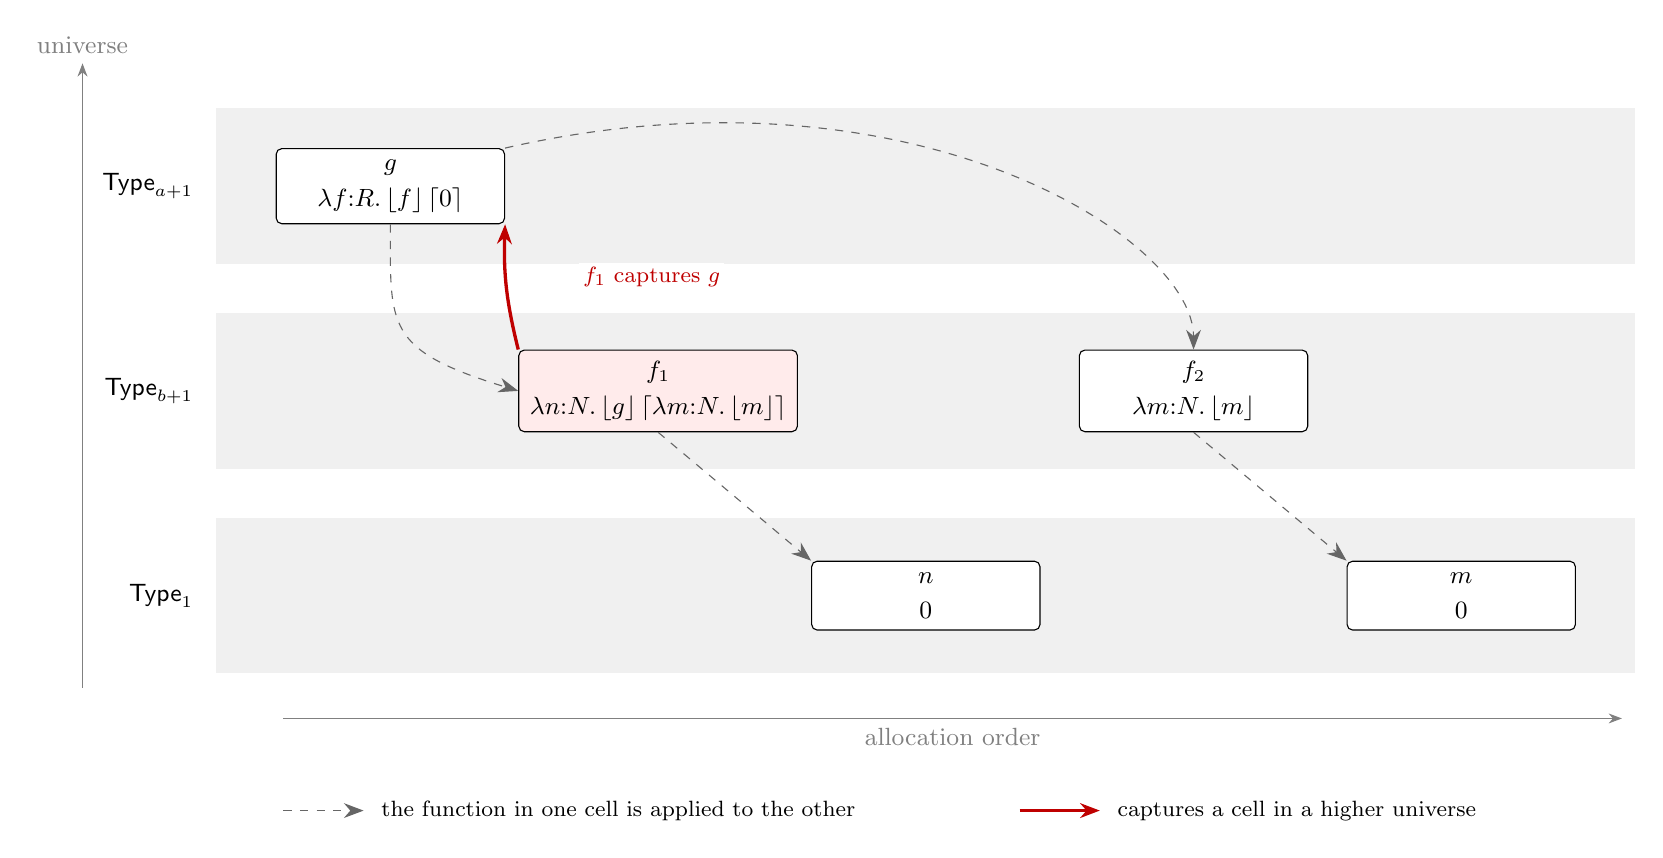
\begin{tikzpicture}[
    x=3.4cm, y=2.6cm,
    cell/.style={draw, rounded corners=2pt, fill=white, align=center,
                 inner sep=4pt, minimum width=2.9cm, font=\small},
    dead/.style={cell, draw=black!35, text=black!45},
    band/.style={fill=black!6, draw=none},
    stored/.style={-{Stealth[length=2.5mm]}, thick},
    arg/.style={-{Stealth[length=2.5mm]}, dashed, black!60},
    bad/.style={stored, red!75!black, line width=1.2pt},
    lbl/.style={font=\footnotesize, fill=white, inner sep=1.5pt},
  ]

  % universe bands, ordered 1 <= c <= b < b+1 <= d <= a < a+1
  \foreach \y/\name in {0/{\Type{1}}, 1/{\Type{b+1}}, 2/{\Type{a+1}}} {
    \fill[band] (0.35, \y - 0.38) rectangle (5.65, \y + 0.38);
    \node[anchor=east, font=\small] at (0.3, \y) {$\name$};
  }
  \draw[-{Stealth}, black!50] (-0.15, -0.45) -- (-0.15, 2.6)
    node[above, font=\small] {universe};
  \draw[-{Stealth}, black!50] (0.6, -0.6) -- (5.6, -0.6)
    node[midway, below, font=\small] {allocation order};

  % cells: x = allocation order, y = universe
  \node[cell] (g)  at (1, 2) {$g$ \\[2pt] $\lam{f}{R} \frc{f}\,\prom{0}$};
  \node[cell, fill=red!8] (c)  at (2, 1)
    {$f_1$ \\[2pt] $\lam{n}{N} \frc{g}\,\prom{\lam{m}{N} \frc{m}}$};
  \node[cell] (z1) at (3, 0) {$n$ \\[2pt] $0$};
  \node[cell] (id) at (4, 1) {$f_2$ \\[2pt] $\lam{m}{N} \frc{m}$};
  \node[cell] (z2) at (5, 0) {$m$ \\[2pt] $0$};

  % the captured variable that breaks stratification: up to a higher universe
  \draw[bad] (c.north west) to[bend left=8] (g.south east);
  \node[lbl, text=red!75!black, align=left, anchor=west]
    at ($(c.north west)!0.5!(g.south east) + (0.25, 0.05)$)
    {$f_1$ captures $g$};

  % applications at run time
  \draw[arg] (g.south) .. controls +(0, -0.5) and +(-0.5, 0.2) .. (c.west);
  \draw[arg] (g.north east) .. controls +(1.5, 0.45) and +(0, 0.55) .. (id.north);
  \draw[arg] (c.south) -- (z1.north west);
  \draw[arg] (id.south) -- (z2.north west);

  % legend
  \begin{scope}[shift={(0.6, -1.05)}]
    \draw[arg] (0, 0) -- (0.3, 0);
    \node[anchor=west, font=\footnotesize] at (0.33, 0)
      {the function in one cell is applied to the other};
    \draw[bad] (2.75, 0) -- (3.05, 0);
    \node[anchor=west, font=\footnotesize] at (3.08, 0)
      {captures a cell in a higher universe};
  \end{scope}
\end{tikzpicture}
\end{center}

\begin{itemize}
  \item $g$ holds $\lam{f}{R} \frc{f}\,\prom{0}$, which captures nothing.
  \item $g$'s function is applied to $f_1$ and then to $f_2$. Both sit in
    $\Type{b+1}$, below $g$, as stratification requires.
  \item Each call forces its $f$ and applies the result to a fresh
    $\prom{0}$: $n$ in the first call, $m$ in the second. Those sit lower
    still, in $\Type{1}$.
  \item $f_1$'s value captures $g$, so it points up, from $\Type{b+1}$ into
    $\Type{a+1}$. This is the highlighted side condition $c \geq a+1$ of the
    derivation.
\end{itemize}
The run-time heap is acyclic. $f_1$ only points to $g$, which was allocated
earlier and holds a value that points nowhere. The problem is that the two
orders disagree: $f_1$ points to the past in time, but into the future in
universes. $g$ must sit above $f_1$ because $g$'s function is applied to $f_1$.
$f_1$ must sit above $g$ because it captures $g$.

\section{Why no levels work}
\label{sec:why}

The highlighted side condition, combined with kinding, gives
\[
  c \;\geq\; a + 1 \;\geq\; d + 1 \;\geq\; b + 2 \;\geq\; c + 2,
\]
which no choice of levels satisfies. Both $+1$s come from the \rn{Promise}
kinding rule, that is, from the $\mathsf{Ref}$ inside a promise:
\begin{itemize}
  \item $d \geq b + 1$: $g$'s argument is a promise, so $\tau_g$ has a
    promise domain.
  \item $c \geq a + 1$: the closure $\lam{n}{N} \cdots$ captures $g$, and $g$
    is a promise.
\end{itemize}
Under the call-by-value translation (the identity) there are no promises, and
$P$ types with every level at $0$ (\S\ref{sec:cbv}).

\paragraph{A less naive translation.}
Suppose a translation passes value arguments directly, and take the case most
favourable to it: $g$'s argument is a plain function, so
$\tau_g = F \arr{d} \Nat$ with $d \geq c$. When $P$ is applied to a
computation, $g$ is still a promise, $T = \Prom{a}{\tau_g}$ with $a \geq d$, and
the closure $\lam{n}{N} \cdots$ still captures it, so $c \geq a + 1$. Then
\[
  c \;\geq\; a + 1 \;\geq\; d + 1 \;\geq\; c + 1.
\]
The gap shrinks from $2$ to $1$, but it never closes.

\newpage
\section{The call-by-value version}
\label{sec:cbv}

Read as a call-by-value $\lambda_{\mathrm{PR}}$ term, $P$ has no references.
It is
\[
  \lam{g}{\tau_g'} g\,(\lam{n}{\Nat} g\,(\lam{m}{\Nat} m))
\]
with the types $F'$ and $\tau_g'$ below. The cycle of constraints is the same
as before, but every edge is non-strict.

\paragraph{Kinding.}

\tree{
  \inferrule*[right={\rn{Arr}\enspace$d \geq c$}]
  {
    \inferrule*[right={\rn{Arr}\enspace$c \geq 0$}]
      {\Nat :: \Type{0} \\ \Nat :: \Type{0}}
      {F' = \Nat \arr{c} \Nat \;::\; \Type{c}}
    \\
    \Nat :: \Type{0}
  }
  {\tau_g' = F' \arr{d} \Nat \;::\; \Type{d}}
}

\paragraph{Typing.}
The highlighted side condition is the one that failed before: the closure
$\lam{n}{\Nat} \cdots$ captures $g$. Now $g$ is a function, not a cell, so the
free-variable rule asks only that $c \geq d$.

\tree{
    \inferrule*[right={$\lambda$\enspace$e \geq d$}]
    {
      \inferrule*
      {
        \inferrule*{ }{g{:}\tau_g' \vdash g : \tau_g'}
        \\
        \inferrule*[right={$\lambda$\enspace$\good{c \geq d}$}]
        {
          \inferrule*
          {
            \inferrule*{ }{g{:}\tau_g', n{:}\Nat \vdash g : \tau_g'}
            \\
            \inferrule*[right={$\lambda$\enspace$c \geq 0$}]
            {
              \inferrule*{ }
                {g{:}\tau_g', n{:}\Nat, m{:}\Nat \vdash m : \Nat}
            }
            {g{:}\tau_g', n{:}\Nat \vdash \lam{m}{\Nat} m : F'}
          }
          {g{:}\tau_g', n{:}\Nat \vdash g\,(\lam{m}{\Nat} m) : \Nat}
        }
        {g{:}\tau_g' \vdash \lam{n}{\Nat} g\,(\lam{m}{\Nat} m) : F'}
      }
      {g{:}\tau_g' \vdash g\,(\lam{n}{\Nat} g\,(\lam{m}{\Nat} m)) : \Nat}
    }
    {\vdash \lam{g}{\tau_g'} g\,(\lam{n}{\Nat} g\,(\lam{m}{\Nat} m)) : \tau_g' \arr{e} \Nat}
}

Kinding gives $d \geq c$ and typing gives $c \geq d$, so $c = d$. Taking
$c = d = e = 0$ satisfies every side condition. Compare the chain of
\S\ref{sec:why}:
\[
  c \;\geq\; d \;\geq\; c
  \qquad\text{versus}\qquad
  c \;\geq\; a + 1 \;\geq\; d + 1 \;\geq\; b + 2 \;\geq\; c + 2.
\]

\newpage
\paragraph{The heap.}
Run the same program:
\[
  (\lam{g}{\tau_g'} g\,
    \underbrace{\colorbox{green!15}{$\displaystyle
      \lam{n}{\Nat} g\,\underbrace{(\lam{m}{\Nat} m)}_{f_2}$}}_{f_1})\;
  \underbrace{(\lam{f}{F'} f\,0)}_{g}
\]
$\lambda_{\mathrm{PR}}$ has no cells here: variables are bound to values. The
figure shows the closures that an implementation allocates on the heap,
named as before, and placed in the universe of their type. Numbers are passed
directly, so $n$ and $m$ get no heap object.

\begin{center}
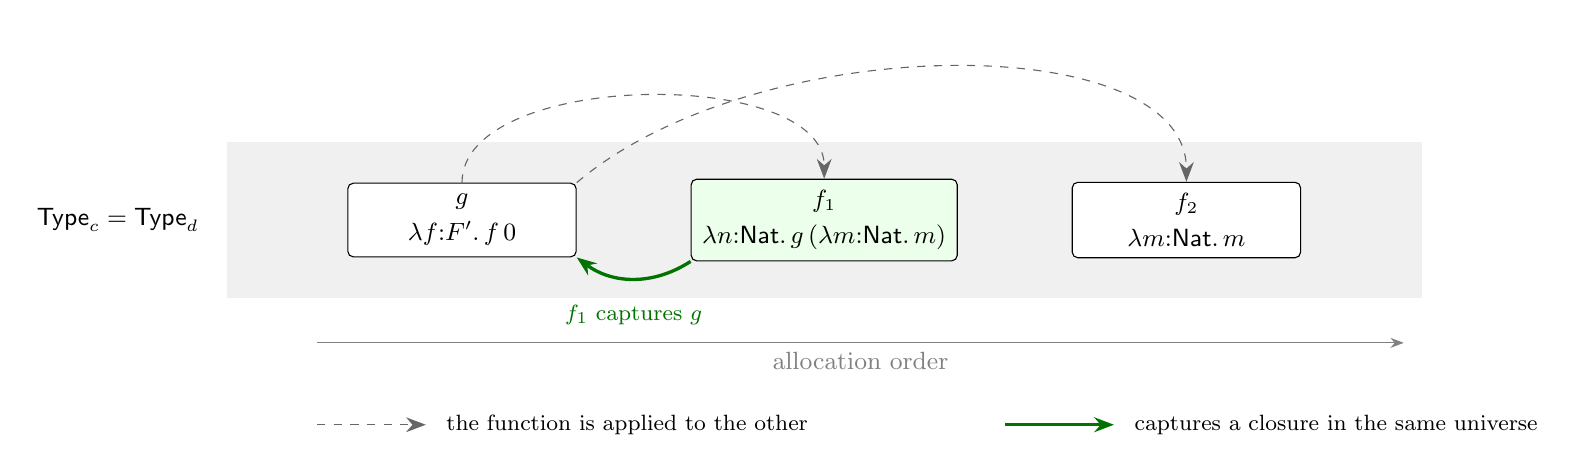
\begin{tikzpicture}[
    x=4.6cm, y=2.6cm,
    cell/.style={draw, rounded corners=2pt, fill=white, align=center,
                 inner sep=4pt, minimum width=2.9cm, font=\small},
    band/.style={fill=black!6, draw=none},
    stored/.style={-{Stealth[length=2.5mm]}, thick},
    arg/.style={-{Stealth[length=2.5mm]}, dashed, black!60},
    ok/.style={stored, green!45!black, line width=1.2pt},
    lbl/.style={font=\footnotesize, fill=white, inner sep=1.5pt},
  ]

  % one universe band: c = d
  \fill[band] (0.35, -0.38) rectangle (3.65, 0.38);
  \node[anchor=east, font=\small] at (0.3, 0) {$\Type{c} = \Type{d}$};
  \draw[-{Stealth}, black!50] (0.6, -0.6) -- (3.6, -0.6)
    node[midway, below, font=\small] {allocation order};

  \node[cell] (g)  at (1, 0) {$g$ \\[2pt] $\lam{f}{F'} f\,0$};
  \node[cell, fill=green!8] (c) at (2, 0)
    {$f_1$ \\[2pt] $\lam{n}{\Nat} g\,(\lam{m}{\Nat} m)$};
  \node[cell] (id) at (3, 0) {$f_2$ \\[2pt] $\lam{m}{\Nat} m$};

  % the captured variable: same universe, which immutable closures allow
  \draw[ok] (c.south west) to[bend left=35] (g.south east);
  \node[lbl, text=green!45!black, anchor=north] at ($(c.south west)!0.5!(g.south east) + (0, -0.2)$)
    {$f_1$ captures $g$};

  % applications at run time
  \draw[arg] (g.north) .. controls +(0, 0.55) and +(0, 0.55) .. (c.north);
  \draw[arg] (g.north east) .. controls +(0.5, 0.75) and +(0, 0.75) .. (id.north);

  % legend
  \begin{scope}[shift={(0.6, -1.0)}]
    \draw[arg] (0, 0) -- (0.3, 0);
    \node[anchor=west, font=\footnotesize] at (0.33, 0)
      {the function is applied to the other};
    \draw[ok] (1.9, 0) -- (2.2, 0);
    \node[anchor=west, font=\footnotesize] at (2.23, 0)
      {captures a closure in the same universe};
  \end{scope}
\end{tikzpicture}
\end{center}

\begin{itemize}
  \item $g$'s function is applied to $f_1$ and then to $f_2$, both in its own
    universe. A function at level $d$ may take an argument at level $c \leq d$.
  \item $f_1$ captures $g$, also in its own universe. A closure at level $c$ may
    capture a value at level $d \leq c$.
\end{itemize}
Both arrows stay inside one universe, so the two orders no longer disagree.
That is allowed because closures are immutable: stratification constrains
only what a reference may hold. In the call-by-need version $f_1$ and $g$ are
cells, so each of these two arrows costs a universe, and they cannot both be
satisfied.

\newpage
\section{A logical relation for promises}
\label{sec:lr}

Both $+1$s in \S\ref{sec:why} come from encoding a promise as a
$\mathsf{Ref}$. But a promise is written only once, and only with the value
of its own thunk. This section makes promises primitive, gives them no level
at all, and proves termination with a Kripke logical relation whose worlds
contain no types. The image of $P$ is typeable, so it terminates.
Everything in this section is mechanized in \texttt{Promises.agda}, using
environments instead of substitution.

\subsection{The language}

The target language has natural numbers, functions and primitive promises,
and no references. Since nothing in it costs a level, there are no level
annotations.
\[
\begin{array}{@{}l@{\quad}r@{\;\;::=\;\;}l@{}}
  \text{Types} & \tau & \Nat \mid \tau \to \tau \mid \Prom{}{\tau} \\
  \text{Values} & v & n \mid \lam{x}{\tau} e \mid \ell \\
  \text{Expressions} & e & v \mid x \mid e\,e \mid \prom{e} \mid \frc{e} \\
  \text{Stores} & S & \cdot \mid S[\ell \mapsto e]
\end{array}
\]
A store maps each location to a closed expression: an unforced thunk, or a
memoized value. The translation of \S2 is unchanged, except that
$\Prom{}{\tau}$, $\prom{e}$ and $\frc{e}$ are now primitive. Typing is
standard, with
\begin{mathpar}
  \inferrule*[right={$\lceil\cdot\rceil$}]
    {\Gamma \vdash e : \tau}
    {\Gamma \vdash \prom{e} : \Prom{}{\tau}}
  \and
  \inferrule*[right={$\lfloor\cdot\rfloor$}]
    {\Gamma \vdash e : \Prom{}{\tau}}
    {\Gamma \vdash \frc{e} : \tau}
\end{mathpar}
With $N = \Prom{}{\Nat}$, $F = N \to \Nat$, $R = \Prom{}{F}$,
$\tau_g = R \to \Nat$ and $T = \Prom{}{\tau_g}$, the derivation of \S4 goes
through with every side condition gone:
$\vdash \tr{P} : T \to \Nat$.

\paragraph{Evaluation.}
Evaluation is big-step and records its trace $\pi$, the list of stores
after each change to the store. Forcing has two rules: a memo hit returns the
stored value without writing, and a memo miss runs the thunk and then writes
its value back.
\begin{mathpar}
  \inferrule{ }{\evals{S}{v}{S}{v}{\varepsilon}}
  \and
  \inferrule
    {\evals{S}{e_1}{S_1}{\lam{x}{\tau} e}{\pi_1} \\
     \evals{S_1}{e_2}{S_2}{v_2}{\pi_2} \\
     \evals{S_2}{e[v_2/x]}{S_3}{v}{\pi_3}}
    {\evals{S}{e_1\,e_2}{S_3}{v}{\pi_1\,\pi_2\,\pi_3}}
  \and
  \inferrule
    {\ell = \fresh(S)}
    {\evals{S}{\prom{e}}{S[\ell \mapsto e]}{\ell}{S[\ell \mapsto e]}}
  \\
  \inferrule*[right=Hit]
    {\evals{S}{e}{S_1}{\ell}{\pi_1} \\ S_1(\ell) = v}
    {\evals{S}{\frc{e}}{S_1}{v}{\pi_1}}
  \and
  \inferrule*[right=Miss]
    {\evals{S}{e}{S_1}{\ell}{\pi_1} \\ S_1(\ell) = t \notin \Val \\
     \evals{S_1}{t}{S_2}{v}{\pi_2}}
    {\evals{S}{\frc{e}}{S_2[\ell \mapsto v]}{v}{\pi_1\,\pi_2\,S_2[\ell \mapsto v]}}
\end{mathpar}
$\fresh$ is a function, such as the least location not in $\mathrm{dom}(S)$,
so evaluation is deterministic.

\subsection{Worlds}

The type-world circularity arises because worlds map locations to types, and
the meaning of a type depends on worlds. Here a world is instead the history
of a computation: the sequence of stores it has passed through. A world
contains no types, so there is nothing circular to define.

\paragraph{Definition.}
A world $W = S_0 \cdots S_n$ is a non-empty sequence of stores in which
each store arises from the previous one by one of two steps:
\begin{itemize}
  \item \emph{allocation}: $S_{i+1} = S_i[\ell \mapsto e]$, with
    $\ell \notin \mathrm{dom}(S_i)$ and $e$ any closed expression;
  \item \emph{memoization}: $S_{i+1} = S_i[\ell \mapsto v]$, where for some
    $j \leq i$, $S_j(\ell) = t \notin \Val$ and
    $\evals{S_j}{t}{S_i}{v}{S_{j+1} \cdots S_i}$.
\end{itemize}
A memoization is justified by a run of the cell's own thunk, recorded
earlier in the same world. That is the only way a cell's contents ever
change. $W' \ext W$ when $W$ is a prefix of $W'$, and $\last{W}$ is the final
store of $W$: the present. Domains only grow along a world, and a cell's contents change
only from a thunk to a value.

\begin{lemma}[Runs extend worlds]
  If $\evals{\last{W}}{e}{S}{v}{\pi}$, then $W \cdot \pi$ is a world.
\end{lemma}
\begin{proof}
  By induction on the derivation. In \rn{Miss}, the final write is a
  memoization justified by the position of $S_1$ in $W \cdot \pi_1$, and by
  the run of $t$, whose trace is exactly $\pi_2$.
\end{proof}

\subsection{The relation}

\[
\begin{array}{@{}l@{\;\;=\;\;}l@{}}
  \Vrel{\Nat}{W} & \mathbb{N} \\
  \Vrel{A \to B}{W} &
    \{\, \lam{x}{A} e \mid \forall W' \ext W.\ \forall v \in \Vrel{A}{W'}.\
      e[v/x] \in \Erel{B}{W'} \,\} \\
  \Vrel{\Prom{}{\tau}}{W} &
    \{\, \ell \in \mathrm{dom}(\last{W}) \mid \forall W' \ext W.\
      \last{W'}(\ell) \in \Erel{\tau}{W'} \,\} \\[1ex]
  \Erel{\tau}{W} &
    \{\, e \mid \forall W' \ext W.\
      \evals{\last{W'}}{e}{S}{v}{\pi} \wedge v \in \Vrel{\tau}{W' \cdot \pi} \,\} \\
  \Grel{\Gamma}{W} &
    \{\, \gamma \mid \forall x{:}A \in \Gamma.\ \gamma(x) \in \Vrel{A}{W} \,\}
\end{array}
\]
The definition is by induction on the type: $\Vrel{\Prom{}{\tau}}{W}$ only
mentions $\Erel{\tau}{\cdot}$, and worlds are syntactic. A promise is good
when its cell's contents, thunk or memoized value, are a good computation in
every future. No other cell's type is ever consulted.

\begin{lemma}[Monotonicity]
  If $W' \ext W$, then $\Vrel{\tau}{W} \subseteq \Vrel{\tau}{W'}$ and
  $\Erel{\tau}{W} \subseteq \Erel{\tau}{W'}$.
\end{lemma}
\begin{proof}
  Every clause quantifies over all extensions, and $\ext$ is transitive.
  Domains only grow, so $\ell \in \mathrm{dom}(\last{W'})$.
\end{proof}

\begin{lemma}[Values]
  $\Vrel{\tau}{W} \subseteq \Erel{\tau}{W}$.
\end{lemma}
\begin{proof}
  A value evaluates to itself with an empty trace. Apply monotonicity.
\end{proof}

\begin{lemma}[History of a cell]
  Let $\ell \notin \mathrm{dom}(\last{W})$, let $W_1 = W \cdot
  \last{W}[\ell \mapsto t]$ with $t \notin \Val$, and let $W^* \ext W_1$. Then
  either $\last{W^*}(\ell) = t$, or $\last{W^*}(\ell) = v$ and $W^*$ has a
  prefix $W_j \cdot \pi \cdot S[\ell \mapsto v]$, where $W_j \ext W_1$,
  $\evals{\last{W_j}}{t}{S}{v}{\pi}$, and $\ell$ is not written afterwards.
\end{lemma}
\begin{proof}
  Take the last memoization of $\ell$ in $W^*$. Its justification is a store
  $S_j$ with $S_j(\ell) \notin \Val$. $S_j$ contains $\ell$, so it comes no
  earlier than $\last{W_1}$, because $\ell$ was fresh. A cell's contents only
  change from a thunk to a value, so $S_j(\ell) = t$.
\end{proof}

\subsection{The fundamental lemma}

\begin{lemma}[Fundamental]
  If $\Gamma \vdash e : \tau$ and $\gamma \in \Grel{\Gamma}{W}$, then
  $\gamma(e) \in \Erel{\tau}{W}$.
\end{lemma}
\begin{proof}
  By induction on the typing derivation. Variables, numbers, $\lambda$ and
  application are standard, using monotonicity and the values lemma. We show
  the two promise cases.

  \emph{Promise.} Let $W' \ext W$, $S' = \last{W'}$ and $t = \gamma(e)$. Then
  $\evals{S'}{\prom{t}}{S_1}{\ell}{S_1}$ with $S_1 = S'[\ell \mapsto t]$ and
  $\ell = \fresh(S')$. Let $W_1 = W' \cdot S_1$. We must show
  $\ell \in \Vrel{\Prom{}{\tau}}{W_1}$, so let $W^* \ext W_1$. By the history
  lemma, there are two cases.
  \begin{itemize}
    \item $\last{W^*}(\ell) = t$. By the induction hypothesis,
      $t \in \Erel{\tau}{W}$, and $W^* \ext W$.
    \item $\last{W^*}(\ell) = v$, from a run
      $\evals{\last{W_j}}{t}{S}{v}{\pi}$ with $W_j \ext W_1 \ext W$. By the
      induction hypothesis, $t \in \Erel{\tau}{W_j}$, and by determinism this
      is the run that relation describes. So
      $v \in \Vrel{\tau}{W_j \cdot \pi}$. Since $W^* \ext W_j \cdot \pi$,
      monotonicity gives $v \in \Vrel{\tau}{W^*}$, and the values lemma gives
      $v \in \Erel{\tau}{W^*}$.
  \end{itemize}

  \emph{Force.} Let $W' \ext W$. By the induction hypothesis,
  $\evals{\last{W'}}{\gamma(e)}{S_1}{\ell}{\pi_1}$ with
  $\ell \in \Vrel{\Prom{}{\tau}}{W_1}$, where $W_1 = W' \cdot \pi_1$. Taking
  the trivial extension, $S_1(\ell) \in \Erel{\tau}{W_1}$.
  \begin{itemize}
    \item \rn{Hit}: $S_1(\ell) = v$ evaluates to itself, so
      $v \in \Vrel{\tau}{W_1}$.
    \item \rn{Miss}: $S_1(\ell) = t$, and
      $\evals{S_1}{t}{S_2}{v}{\pi_2}$ with $v \in \Vrel{\tau}{W_1 \cdot \pi_2}$.
      The final world $W_1 \cdot \pi_2 \cdot S_2[\ell \mapsto v]$ extends
      $W_1 \cdot \pi_2$, so monotonicity finishes the case. \qedhere
  \end{itemize}
\end{proof}

\paragraph{Corollary.}
Every closed, well-typed expression terminates. In particular,
$\tr{P}$ and $\tr{P}\,\prom{(\slam{h} h)\,(\slam{f} f\,0)}$ do.

\subsection{Remarks}

\begin{itemize}
  \item \emph{Acyclicity is a consequence, not an assumption.} Nothing above
    says that a thunk cannot reach its own cell. If it did, forcing it would
    re-enter the cell forever, and the thunk would not be in
    $\Erel{\tau}{\cdot}$. The fundamental lemma shows that no well-typed
    thunk does this.
  \item \emph{Why this fails for references.} The proof works because a
    memoization is justified by evaluation: the world records the run
    that produced the value, and the cell's own invariant says that run ends
    in a good value. An arbitrary write $\ell \assign v$ has no such
    justification. To keep the cell's invariant, worlds would have to
    allow only writes of values in $\Vrel{\tau}{\cdot}$ at the cell's type
    $\tau$. Worlds would then mention the relation at arbitrary types, and
    the circularity returns. $\lambda_{\mathrm{PR}}$ breaks it with levels.
  \item \emph{Adding references back.} Combining this relation with
    $\lambda_{\mathrm{PR}}$'s levelled worlds is open. A thunk may read a
    reference, so the run that justifies a memoization must start from a heap
    that satisfies the reference world. Stating that inside the definition of
    worlds mentions heap satisfaction, which mentions the relation at
    every level.
\end{itemize}

\section{Why no shallow model covers STLC}
\label{sec:obstruction}

The original goal was a shallow embedding of call-by-need STLC in Agda.
Types are Agda types, terms are Agda functions, the heap holds semantic
values, and everything is total by structural recursion. The heap is
unobservable to programs. What we want to see is its behaviour: what is
allocated and when, and what is forced. \texttt{Stratified.agda} achieves this
for a fragment. This section explains why no choice of worlds extends it to
all of STLC, and why \S\ref{sec:lr} puts syntax in the heap instead.

\paragraph{The domain equation is the type-world circularity.}
A shallow model with a heap has the shape
\[
\begin{array}{@{}l@{\;\;=\;\;}l@{}}
  \mathit{Comp}\,\tau\,W & \mathit{Heap}\,W \to
    \Sigma\,W' \ext W.\ \mathit{Heap}\,W' \times \mathit{Val}\,\tau\,W' \\
  \mathit{Heap}\,W & \prod_{(\ell : \sigma) \in W}
    \mathit{Val}\,\sigma\,W \uplus \mathit{Comp}\,\sigma\,W \\
  \mathit{Val}\,(A \to B)\,W & \forall W' \ext W.\
    \mathit{Loc}\,W'\,A \to \mathit{Comp}\,B\,W'
\end{array}
\]
$\mathit{Heap}$ occurs negatively in its own definition. Even when $W$ is
syntactic, as in \texttt{Stratified.agda}, $\mathit{Heap}\,W$ is the
interpretation of $W$, cell by cell. This is Ahmed's equation, with the
heap's type playing the semantic world:
\[
  \mathit{Type} = \mathit{World} \to \mathcal{P}(\mathit{Val})
  \quad\sim\quad \mathit{Comp}\ \text{reads}\ \mathit{Heap},
  \qquad
  \mathit{World} = \mathit{Loc} \rightharpoonup \mathit{Type}
  \quad\sim\quad \mathit{Heap}\,W = \textstyle\prod_\ell
    \llbracket W(\ell) \rrbracket.
\]
Agda accepts such a definition only with a well-founded measure that
decreases from a cell's domain to the heaps that domain reads. Levels are
such a measure: $\mathit{Heap}_{k+1}$ contains only $\mathit{Val}_k$ and
$\mathit{Comp}_k$.

\paragraph{The counterexample defeats every measure.}
Run $P$ on $\slam{f} f\,0$, as in \S5, and write $D(x)$ for the Agda type
interpreting the contents of cell $x$.
\begin{itemize}
  \item $g$ holds a function that forces its argument $f_1$, so $D(g)$ takes
    heaps containing $f_1$: $\mu(g) > \mu(f_1)$.
  \item $f_1$ holds a thunk that forces $g$, so $D(f_1)$ takes heaps
    containing $g$: $\mu(f_1) > \mu(g)$.
\end{itemize}
Both inequalities come from the definitions of the domains, not from any
particular run.

\paragraph{Capture versus use.}
The history is stratified: every pointer out of a cell points to that cell's
past (\S5, \S\ref{sec:lr}). But that orders what a cell's contents
\emph{capture}. Defining $D$ needs what they \emph{do}, and functions are
applied in the future. $g$'s function captures nothing, yet it is applied to
$f_1$, which is created after $g$ and reads $g$. Suppose $g$'s contents were
interpreted in a world containing only cells up to $g$. Then $g$'s function
could only be applied to cells up to $g$, which is exactly
$\lambda_{\mathrm{PR}}$'s restriction, and the chain of \S\ref{sec:why}
returns.

\paragraph{Fixes that fail.}
\begin{itemize}
  \item \emph{Measure by type.} $f_1 : F$ reads $g : \tau_g$, a larger type.
  \item \emph{Measure by allocation time or dependency position.} These grow
    with the history, and the future is unbounded.
  \item \emph{Levels chosen at run time and recorded in the world.} $g$'s
    value, and so its level, is fixed before $f_1$ exists. $f_1$ must sit
    above $g$'s cell, out of reach of $g$'s function.
  \item \emph{Separate structures for forced and unforced cells.} The cycle
    passes through both: when $g$'s function is applied, $g$ is forced and
    $f_1$ is not.
  \item \emph{Level-polymorphic stored functions.} This is impredicative. In
    Agda, such a value lives in $\mathsf{Set}\omega$, and no cell can hold
    it. An impredicative universe does not help, because the equation is not
    positive, and impredicativity is inconsistent with
    non-strictly-positive inductive types (Coquand and Paulin-Mohring).
  \item \emph{One copy of $g$ per use.} That is call-by-name: two cells
    where call-by-need has one.
\end{itemize}
Execution, unlike definition, is well-founded. Forcing a cell runs only on
its dependency prefix and the cells it allocates, so even the inner call of
$g$'s function, inside the forcing of $f_1$, happens in a world without
$f_1$. But $D(g)$ must also cover the outer call, which happens in a world
containing $f_1$. \S\ref{sec:lr} exploits the well-founded execution and
never defines $D$.

\paragraph{What remains.}
\begin{itemize}
  \item \emph{The stratified fragment.} \texttt{Stratified.agda} is shallow
    and total on the programs whose translation $\lambda_{\mathrm{PR}}$
    accepts, if the conjecture of STRATIFIED.md holds.
  \item \emph{A budget.} An index that shrinks as the history grows, such as
    the number of forces remaining, is well-founded. It gives a shallow,
    total model with a $\mathit{timeout}$ outcome. Showing that some budget
    always suffices needs the relation of \S\ref{sec:lr}. Guarded recursion
    is the type-theoretic form of the same idea, and its results arrive
    under a later modality.
  \item \emph{Syntax in the heap.} Cells hold codes, and the meaning of a code
    is supplied by the type of the pointer to it (\S\ref{sec:lr},
    \texttt{Promises.agda}). Terms are deep, but the relation is defined by
    structural recursion on types, and \texttt{run} is a total evaluator.
  \item \emph{No heap.} Promises interpreted as $\Unit \to \tau$, or
    call-by-need as clairvoyant call-by-value (Hackett and Hutton). Both are
    shallow and total, but neither has cells to allocate.
\end{itemize}
We take syntax in the heap. Each world records every allocation and every
memoization, so the allocation behaviour is visible, and
\texttt{Promises.agda} checks it for $P$: six cells, five forced, one never
forced. Deallocation is not modelled yet.

\section{Worlds compared}
\label{sec:worlds}

The type-world circularity has the same source in every model of
higher-order state: a world must say what each cell may hold, and if that
description is semantic, it depends on worlds. This section compares how
four models avoid it. They are $\lambda_{\mathrm{PR}}$; the core and extended
$L^3$ of Ahmed, Fluet and Morrisett (\emph{$L^3$: A Linear Language with
Locations}, 2007); the full ground references of Kammar, Levy, Moss and
Staton (\emph{A Monad for Full Ground Reference Cells}, LICS 2017); and the
worlds of \S\ref{sec:lr}.

\paragraph{What a world records.}
\begin{itemize}
  \item $\lambda_{\mathrm{PR}}$: a map from locations to a level and a
    \emph{semantic} type, $\mathit{World}_{k+1} = \mathit{Loc}
    \rightharpoonup (i : \mathit{Fin}(k+1)) \times \mathit{Type}_i$. The
    circularity is cut by levels: a world at level $k$ only mentions types
    below $k$.
  \item Core $L^3$: no world at all. A type means a set of pairs $(\sigma, v)$
    of a value and its \emph{exclusive store}, the concrete part of the
    store it owns. $\mathsf{Cap}\,\ell\,\tau$ means
    $\{(\sigma + \{\ell \mapsto v\}, \mathsf{cap}) \mid (\sigma, v) \in
    \mathcal{V}\llbracket\tau\rrbracket\}$, so the definition is by
    induction on types.
  \item Extended $L^3$, which adds ML-style references: a store typing
    $\Psi$ from frozen locations to semantic types. That brings the
    circularity back, and $L^3$ cuts it with step-indexing, consulting
    $\Psi$ only at a smaller approximation, $\lfloor\Psi\rfloor_j$ with
    $j < k$. Step indices play the role that levels play in
    $\lambda_{\mathrm{PR}}$.
  \item Full ground references: a \emph{heap layout}
    $w : \mathit{Loc} \rightharpoonup_{\mathit{fin}} \mathit{Sort}$, mapping
    each location to the \emph{syntactic} name of a full ground type. Types
    denote functors from worlds to sets, with
    $\llbracket \mathsf{ref}\,c \rrbracket w = \{\ell \mid w(\ell) = c\}$.
  \item \S\ref{sec:lr}: the whole history of concrete stores, with no types.
\end{itemize}

Full ground references and \S\ref{sec:lr} both avoid the circularity by
making worlds syntactic, but they restrict different things. Full ground
references restrict \emph{what} a cell may hold: data and references, never
functions or thunks. A cell's meaning at a world then depends only on that
world. In the paper's words, when initialising a cell, ``all the information
we need in order to determine its value is in the target world''. Promises
restrict \emph{how} a cell may change: once, by its own thunk. Contents may be
higher-order. Their meaning is not recorded in the world, but carried by the
pointer's type, as in core $L^3$.

\paragraph{Allocation.}
\begin{itemize}
  \item $\lambda_{\mathrm{PR}}$: extend the world with the new location and
    the semantic type of its contents, at a lower level.
  \item Core $L^3$: the new cell joins the exclusive store of the value that
    owns it. The rest of the store is untouched.
  \item Full ground references: heaps
    $H w = \prod_{(\ell : c) \in w} \llbracket \mathit{ctype}\,c \rrbracket w$
    are not functorial in layout extension. A heap at $w$ cannot be turned
    into a heap at a larger $w'$ without values for the new cells. So a world
    morphism is not just an injection. In the category of
    \emph{initialisations}, a morphism $w_1 \to w_2$ is an injection together
    with a heaplet giving the initial contents of the new cells, which may
    refer to each other cyclically. Heaps are functorial over
    initialisations, as the representable $H \cong E(\emptyset, -)$.
  \item \S\ref{sec:lr}: an allocation step appends a store with the new cell
    and its thunk.
\end{itemize}

Our worlds carry their initialisation data, as Kammar et al.'s morphisms do,
but in the objects rather than the morphisms. A history records every store,
so the contents of new cells are already in the larger world, and extension
can be a preorder (the prefix order) instead of a category. The definition
of worlds also allows a cyclic initialisation, a thunk that mentions its own
cell. Evaluation never creates one, because a thunk is built before its cell
exists, and the fundamental lemma never needs to certify one.

\paragraph{Updates.}
\begin{itemize}
  \item $\lambda_{\mathrm{PR}}$: any write of a value of the cell's semantic
    type. The world is unchanged, and the heap must still satisfy it,
    $\mathbf{W} \vdash h$.
  \item Core $L^3$: a strong update by the owner of the capability. Ownership
    is linear, so nothing else can observe the change, and the frame
    condition of $\mathcal{C}\llbracket\tau\rrbracket$ says the rest of the
    store is unmodified.
  \item Full ground references: any well-sorted write. The layout is
    unchanged. Because contents are first-order, every sort-respecting
    assignment is a heap, so there is no satisfaction relation to maintain.
  \item \S\ref{sec:lr}: memoization only, recorded as a step of the world,
    justified by a run of the cell's own thunk recorded earlier in the same
    world.
\end{itemize}

\paragraph{The future.}
$\lambda_{\mathrm{PR}}$, full ground references and \S\ref{sec:lr} quantify
functions over future worlds. These are extensions of the layout for
$\lambda_{\mathrm{PR}}$ and full ground references (ends over
$w \downarrow u$ in the functor category), and extensions of the history
here. Core $L^3$ replaces future worlds with the frame: a computation must
work for every disjoint rest of the store, and leave it unchanged. Promises
cannot use a frame, because cells are shared. The continuation's cells may be
memoized by the computation. Monotonicity of the relation over histories
plays the frame's role: whatever the computation memoizes, every promise that
was good before stays good.

\paragraph{Heaps and worlds.}
In $\lambda_{\mathrm{PR}}$ and full ground references, the heap is separate
from the world and must be related to it: by satisfaction in
$\lambda_{\mathrm{PR}}$, and by typing $H w$ in full ground references. In
core $L^3$ the store fragment is part of the meaning of each value. Here
there is no separate heap: the present heap is $\last{W}$, and the world is
that heap together with its past.

\begin{center}
\small
\begin{tabular}{@{}p{2.6cm}p{4.1cm}p{4.1cm}p{4.1cm}p{4.1cm}@{}}
  & $\lambda_{\mathrm{PR}}$ & $L^3$ (core / extended)
  & full ground references & promises (\S\ref{sec:lr}) \\ \hline
  world & locations $\mapsto$ level and semantic type
    & none / store typing of semantic types
    & layout: locations $\mapsto$ syntactic sort
    & history of concrete stores \\
  cut circularity by & universe levels
    & induction on types / step-indexing
    & first-order contents & syntactic worlds, self-justified writes \\
  what cells hold & anything, at a lower level
    & anything & full ground data & any thunk or value \\
  allocation & extend world
    & extend exclusive store & initialisation (injection and heaplet)
    & append a store \\
  writes & any value of the type
    & strong update by owner / any value of the type
    & any well-sorted value & memoization, justified by a recorded run \\
  aliasing & yes & no (caps linear) / yes & yes & yes \\
  cycles in the heap & no knot, by levels & pointers only / yes & yes (cyclic data)
    & never created
\end{tabular}
\end{center}

\section{Related work}

\paragraph{$L^3$ and full ground references.}
\S\ref{sec:worlds} compares their worlds with ours in detail. Core $L^3$
shares our idea that a cell's invariant is carried by the type of the pointer
to it. Full ground references share our syntactic worlds and our treatment
of allocation data as part of world extension.

\paragraph{$\lambda_{\mathrm{PR}}$.}
Koronkevich and Bowman (\emph{Type Universes as Kripke Worlds}, ICFP 2025)
break the type-world circularity for general references by stratifying
worlds with universe levels. \S\ref{sec:why} shows that encoding promises as
references in $\lambda_{\mathrm{PR}}$ rules out $P$. \S\ref{sec:lr} shows
that promises need no levels, because their only write is justified by
evaluation rather than by a type.

\end{document}
